\documentclass{article}
% Hasse diagram of the elusive seven element lattice.
% Compile with: pdflatex L7.tex
\usepackage{tikz}
\newcommand\dotsize{1pt}
\begin{document}
%----
\begin{center}
  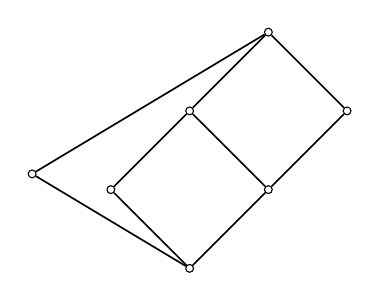
\begin{tikzpicture}[scale=1]
    \node (G) at (2,3) [draw,circle,inner sep=\dotsize] {}; % top
    \node (H) at (1,0) [draw,circle,inner sep=\dotsize] {}; % bottom
    \node (K) at (-1,1.2) [draw,circle, inner sep=\dotsize] {}; % wing
    \node (J1) at (0,1) [draw,circle,inner sep=\dotsize] {};
    \node (M2) at (1,2) [draw,circle,inner sep=\dotsize] {};
    \node (J2) at (2,1) [draw,circle,inner sep=\dotsize] {};
    \node (M1) at (3,2) [draw,circle,inner sep=\dotsize] {};
    \draw[semithick] (H) to (J1) to (M2) to (G) to (M1) to (J2) to (H); 
    \draw[semithick] (J2) to (M2) (H) to (K) to (G);
  \end{tikzpicture}
\end{center}
%----
\end{document}

